\documentclass[11pt, oneside]{article}   	% use "amsart" instead of "article" for AMSLaTeX format
\usepackage{geometry}                		% See geometry.pdf to learn the layout options. There are lots.
\geometry{letterpaper}                   		% ... or a4paper or a5paper or ... 
%\geometry{landscape}                		% Activate for rotated page geometry
%\usepackage[parfill]{parskip}    		% Activate to begin paragraphs with an empty line rather than an indent
\usepackage{graphicx}				% Use pdf, png, jpg, or eps§ with pdflatex; use eps in DVI mode
								% TeX will automatically convert eps --> pdf in pdflatex		
\usepackage{wrapfig}								
\usepackage{amssymb}
%SetFonts
%SetFonts
\date{}							% Activate to display a given date or no date

\begin{document}

\begin{wrapfigure}[0]{r}{0.5\textwidth}
\centering
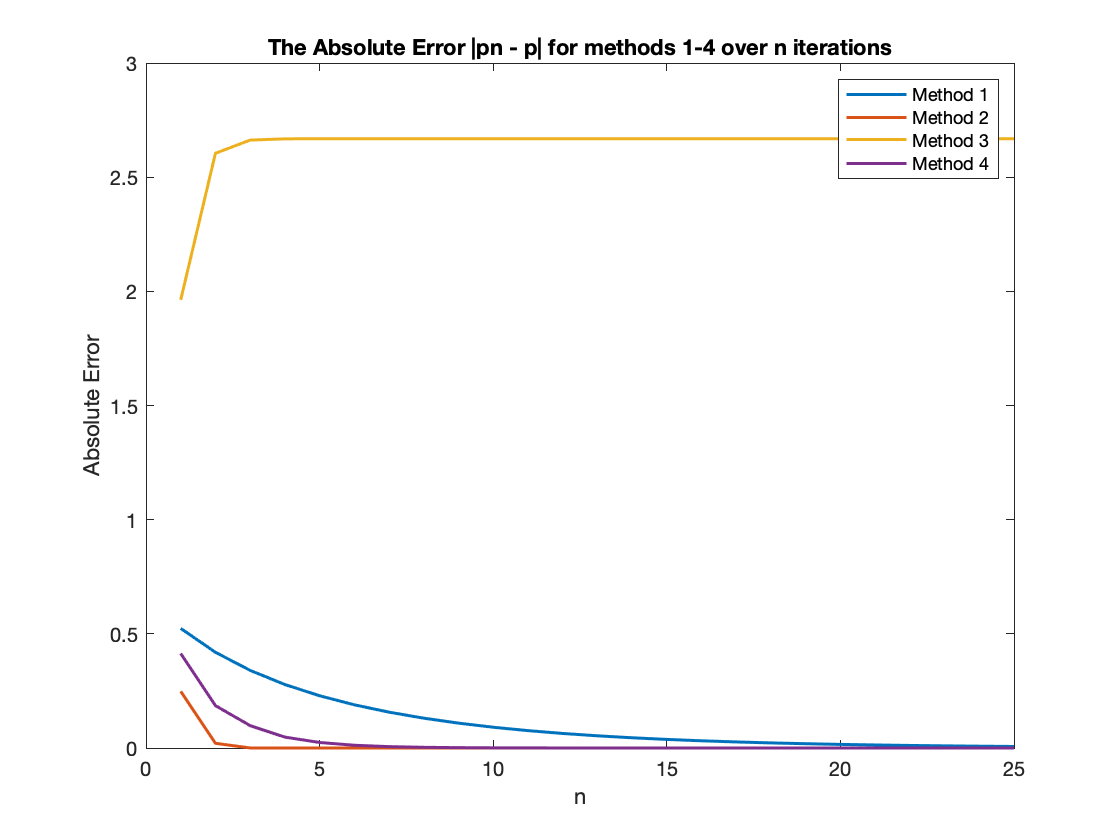
\includegraphics [scale=.18] {Plot_Abs_Error.png}
\end{wrapfigure}

\subsubsection*{Part A}

1. Method 2\\
2. Method 4\\
3. Method 3\\
4. Method 1

$~~~~~$
\\

\subsubsection*{Part B}

\begin{wrapfigure}[8]{r}{0.5\textwidth}
\centering
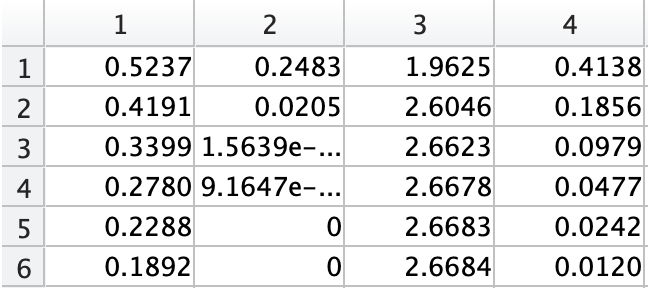
\includegraphics [scale=.54] {Table_AbsErrors.png}
\end{wrapfigure}

Methods 1, 2, and 4 are set up as fixed-point problems: they search for where $g(x) = x$. The fewer iterations required for their absolute errors to equal 0, the faster the convergence. So we see from the graph that method 2 converges fastest, then method 4, then method 1.
\\
Method 3 is a root-finding problem of the form $f(x) = g(x) - x = 0$ where $g(x) = x$. Since $p_n = 0$, $|p_n - p| = | 0 - p | = p$. Once the absolute error for method 3 converges to a value, the solution has been found. Here it has found the root to 5 significant digits after the $6^{th}$ iteration from the table of absolute error values. Similarly, method 2 converged to a solution by the $5^{th}$ iteration.

\subsubsection*{Part C}

Asymptotic error constants were computed using elementwise division and power operations. $p_{n}$ and $p_{n+1}$ are the extraction of all columns and the $2^{nd} : n^{th}$ rows and $1^{st} : n-1^{th}$ rows of the absolute error matrix, respectively. $\lambda$'s for $n = 2:n-1$ were computed.

\begin{itemize}

\item Method 1: For $n \ge 192$, $\alpha = 1$, $\frac{|p_{n+1} - p|}{{|p_n - p|}^\alpha} = 1$. So, this sequence converges to $p$ of order $1$ with asymptotic error constant $\lambda = 1$.

\item Method 2: For $n \ge 5$, $\alpha = 1$, $\frac{|p_{n+1} - p|}{{|p_n - p|}^\alpha} = \frac{0}{0}$, which is undefined.

\item Method 3: For $n \ge 17$, $\alpha = 2$, $\frac{|p_{n+1} - p|}{{|p_n - p|}^\alpha} = 0.374756176784315$. So, this sequence converges to $p$ of order $2$ with asymptotic error constant $\lambda = 0.374756176784315$, and this sequence is said to be quadratically convergent.

\item Method 4: For $n \ge 52$, $\alpha = 1$, $\frac{|p_{n+1} - p|}{{|p_n - p|}^\alpha} = \frac{0}{0}$, which is undefined.

\end{itemize}
\end{document}  